\documentclass{article}
\usepackage{geometry}
 \geometry{
 letterpaper,
 left=1in,
 right=1in,
 top=1in,
 bottom=1in,
 }
\usepackage[utf8]{inputenc}
\usepackage[T1]{fontenc}

\usepackage{amsmath,float}
\floatplacement{figure}{H}
\usepackage{hyperref}
\usepackage{tikz,pgfplots}
\pgfplotsset{compat=1.12}

\graphicspath{{./images/}}
%% Commande supplémentaire

% semi-norm of a vector
\newcommand{\snorm}[1]{\left| #1 \right|}
% norm of a vector
\newcommand{\norm}[1]{\left\| #1 \right\|}
% degree symbol
\newcommand{\degree}[0]{^\circ} 
% rename builtin command \v{} to \vaccent{}
\let\vaccent=\v 
% for vectors
\renewcommand{\v}[1]{\ensuremath{\mathbf{#1}}} 
% for vectors of Greek letters
\newcommand{\gv}[1]{\ensuremath{\mbox{\boldmath$ #1 $}}} 
% for unit vector
\newcommand{\uv}[1]{\ensuremath{\mathbf{\hat{#1}}}}	
% for tensors
%\newcommand{\tn}[1]{\ensuremath{\pmb{\mathsf{#1}}}} 
% for tensors of Greek letters
\newcommand{\tn}[1]{\ensuremath{\mbox{\boldmath$\mathsf{#1}$}}} 
% for absolute value
\newcommand{\abs}[1]{\left| #1 \right|}	
% for average
\newcommand{\avg}[1]{\left< #1 \right>} 
% rename builtin command \d{} to \underdot{}
\let\underdot=\d 
% for derivatives
\renewcommand{\d}[2]{\frac{d #1}{d #2}} 
% for double derivatives
\newcommand{\dd}[2]{\frac{d^2 #1}{d #2^2}} 
% for partial derivatives
\newcommand{\pd}[2]{\frac{\partial #1}{\partial #2}}
% for double partial derivatives
\newcommand{\pdd}[2]{\frac{\partial^2 #1}{\partial #2^2}} 
% for crossed double partial derivatives
\newcommand{\pdx}[3]{\frac{\partial^2 #1}{\partial #2 \partial #3}} 
% for thermodynamic partial derivatives
\newcommand{\pdc}[3]{\left( \frac{\partial #1}{\partial #2} \right)_{#3}} 
% for Dirac bras
\newcommand{\ket}[1]{\left| #1 \right>} 
% for Dirac kets
\newcommand{\bra}[1]{\left< #1 \right|} 
% for Dirac brackets
\newcommand{\braket}[2]{\left< #1 \vphantom{#2} \right| \left. #2 \vphantom{#1} \right>} 
% for Dirac matrix elements
\newcommand{\matrixel}[3]{\left< #1 \vphantom{#2#3} \right| #2 \left| #3 \vphantom{#1#2} \right>} 
% for gradient
\newcommand{\grad}[1]{\gv{\nabla} #1}
% rename builtin command \div to \divsymb
\let\divsymb=\div 
% for divergence
\renewcommand{\div}[1]{\gv{\nabla} \cdot #1} 
% for curl
\newcommand{\curl}[1]{\gv{\nabla} \times #1} 
% for laplacian
\newcommand{\lap}[1]{\gv{\nabla}^2 #1}
% Math text
\newcommand{\mt}[1]{\mathrm{#1}} 
% Overline
\newcommand{\ol}[1]{\overline{#1}}
% Partial derivative with dfrac
\newcommand{\dpd}[2]{\dfrac{\partial #1}{\partial #2}}
% Scientific notation
\providecommand{\e}[1]{\ensuremath{\times 10^{#1}}}
% Symbole degré
\renewcommand{\deg}{$^{\circ}\;$}

% text style
%
\newcommand{\Ae}{\text{\normalshape a.e.}}
% c'est-à-dire
\newcommand{\ie}{\textit{i.e.}\ }
% e.g. - par exemple
\newcommand{\eg}{\textit{e.g.}\ }
\newcommand{\strong}{\text{\normalshape -strong}}
\newcommand{\weak}{\text{\normalshape -weak}}
\newcommand{\loc}{\text{\normalshape loc}}
\newcommand{\ad}{\text{\normalshape ad}}
% Symbole degré
\renewcommand{\deg}{$^{\circ}\;$}
% Accronymes
\newcommand{\PIV}{\textit{PIV}\ }

% Space operator
\newcommand{\Def}{\overset{\text{\textup{def}}}{=}}
\newcommand{\R}{\operatorname{\mathbb R}}
\newcommand{\Rn}{\operatorname{{\mathbb R}^N}}
\newcommand{\RK}{\operatorname{{\mathbb R}^K}}
\newcommand{\N}{\operatorname{\mathbb N}}
\newcommand{\Z}{\operatorname{\mathbb Z}}
\newcommand{\ON}{\operatorname{\text{\textup{O(N)}}}}
\newcommand{\opt}{\mathrm{opt}}

% Matrix operator
\newcommand{\transp}{\:{}^*\,\negmedspace}
\newcommand{\trans}{\:{}^* \negmedspace}
\newcommand{\transm}{\:{}^* \!\negmedspace}
\newcommand{\tran}{{}^* \negmedspace}

% Environnement pour les Théorème, lemmes et remarques
\newtheorem{theoreme}{Th\'{e}or\`{e}me}
\newtheorem{lemme}{Lemme}
\newtheorem{remarque}{Remarque}
\newtheorem{prop}{Proposition}
\newtheorem{hypo}{Hypoth\`{e}se}
\newtheorem{dfn}{D\'{e}finition}

% Variables
\newcommand{\constant}[1]{\mathit{#1}}
\renewcommand\Re{\constant{Re}}  % Reynolds number
\newcommand\Pe{\constant{Pe}}  % Peclet number
\newcommand\Nu{\constant{Nu}}  % Nusselt number
\newcommand\Sh{\constant{Sh}}  % Sherwood number
\newcommand\Sc{\constant{Sc}}  % Schmidt number
\renewcommand\Pr{\constant{Pr}}  % Prandlt number
% Trucs de chimie
\newcommand\el{\mathrm{e^-}}
\newcommand*\chem[1]{\ensuremath{\mathrm{#1}}}

% used tikz libraries
\usetikzlibrary{patterns}
\usetikzlibrary{arrows}
\usetikzlibrary{calc}
\usetikzlibrary{intersections}
\usetikzlibrary{trees}
\usetikzlibrary{positioning}
\usetikzlibrary{arrows}
\usetikzlibrary{chains}
\usetikzlibrary{decorations.shapes}
\usetikzlibrary{decorations.pathreplacing}
\usetikzlibrary{decorations.pathmorphing}
\usetikzlibrary{decorations.markings}
\usetikzlibrary{shapes}
\usetikzlibrary{matrix}

\begin{document}


\begin{figure}[!ht]
\centering
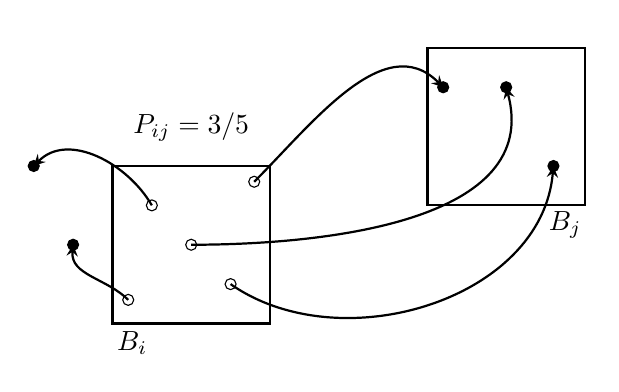
\begin{tikzpicture}
    % two bins
	\draw[thick] (0,0) rectangle (2,2);
	\draw[thick] (4,1.5)   rectangle (4+2,1.5+2);	
	\node at (0.25, -0.25) {$B_i$};
	\node at (5.75, 1.25) {$B_j$};
	\node at (1, 2.5) {$P_{ij} = 3/5$};
	
	% particles def
    \coordinate (A0) at (1.8, 1.8);
    \coordinate (AT) at (4.2, 3);
    \draw (A0) circle (0.07cm);
    \draw[fill=black] (AT) circle (0.07cm);
    
    \coordinate (B0) at (1, 1);
    \coordinate (BT) at (5, 3);
    \draw (B0) circle (0.07cm);
    \draw[fill=black] (BT) circle (0.07cm);
    
    \coordinate (C0) at (1.5, 0.5);
    \coordinate (CT) at (5.6, 2);
    \draw (C0) circle (0.07cm);
    \draw[fill=black] (CT) circle (0.07cm);
    
    \coordinate (D0) at (0.5, 1.5);
    \coordinate (DT) at (-1, 2);
    \draw (D0) circle (0.07cm);
    \draw[fill=black] (DT) circle (0.07cm);
    
    \coordinate (E0) at (0.2, 0.3);
    \coordinate (ET) at (-0.5, 1);
    \draw (E0) circle (0.07cm);
    \draw[fill=black] (ET) circle (0.07cm);
	
	\draw[thick,->,>=stealth] (A0) to [out=45, in=135] (AT);	
	\draw[thick,->,>=stealth] (B0) to [out=0, in=-75] (BT);	
	\draw[thick,->,>=stealth] (C0) to [out=-35, in=-95] (CT);
	\draw[thick,->,>=stealth] (D0) to [out=120, in=45] (DT);
	\draw[thick,->,>=stealth] (E0) to [out=135, in=-95] (ET);	
\end{tikzpicture}
\end{figure}


\begin{figure}[!ht]
\centering
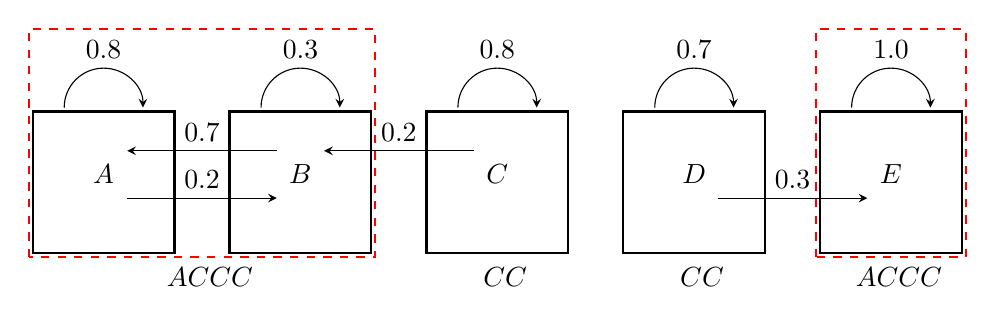
\begin{tikzpicture}
	\draw[color=red,dashed,thick] (0.45,0.45) rectangle (4.85,3.35);
	\draw[color=red,dashed,thick] (10.45,0.45) rectangle (12.35,3.35);
	
	\foreach \x in {0.5, 3, 5.5, 8, 10.5} {
	 \draw[thick] (\x,0.5) rectangle (\x+1.8,2.3);
	}
	
	% letters
	\node at (1.4, 1.5) {$A$}; 
	\node at (3.9, 1.5) {$B$}; 
	\node at (6.4, 1.5) {$C$}; 
	\node at (8.9, 1.5) {$D$}; 
	\node at (11.4, 1.5) {$E$};
	
	% Classes
	\node at (2.75, 0.2) {$ACCC$}; 
	\node at (6.5, 0.2) {$CC$}; 
	\node at (9, 0.2) {$CC$};
	\node at (11.5, 0.2) {$ACCC$};
	
	% arrow
	\draw[->,>=stealth] (1.7, 1.2) -- (3.6, 1.2) node[midway, above] {0.2};
	\draw[<-,>=stealth] (1.7, 1.8) -- (3.6, 1.8) node[midway, above] {0.7};
	
	\draw[<-,>=stealth] (4.2, 1.8) -- (6.1, 1.8) node[midway, above] {0.2};

	\draw[->,>=stealth] (9.2, 1.2) -- (11.1, 1.2) node[midway, above] {0.3};
	\draw[->,>=stealth] (1.4, 1.5)+(-0.5, 0.85) arc (180:0:0.5) node[midway,above] {$0.8$};
	\draw[->,>=stealth] (3.9, 1.5)+(-0.5, 0.85) arc (180:0:0.5) node[midway,above] {$0.3$};
	\draw[->,>=stealth] (6.4, 1.5)+(-0.5, 0.85) arc (180:0:0.5) node[midway,above] {$0.8$};
	\draw[->,>=stealth] (8.9, 1.5)+(-0.5, 0.85) arc (180:0:0.5) node[midway,above] {$0.7$};
	\draw[->,>=stealth] (11.4, 1.5)+(-0.5, 0.85) arc (180:0:0.5) node[midway,above] {$1.0$};
\end{tikzpicture}	
\end{figure}

\begin{figure}[!ht]
\centering
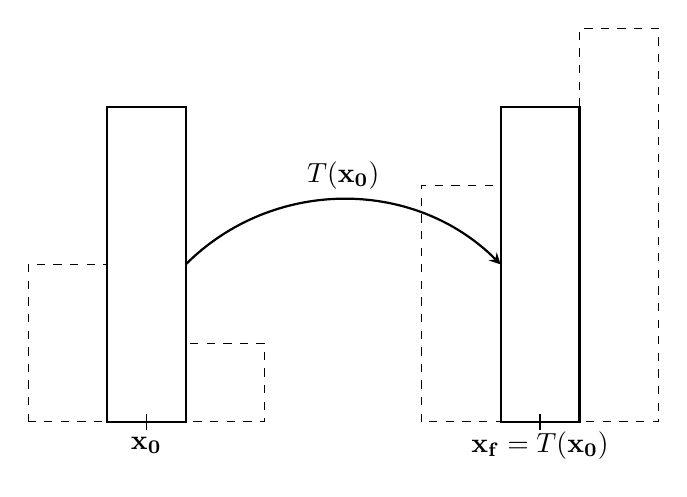
\begin{tikzpicture}
  \draw[dashed] (-1,0) rectangle (0,2);
  \draw[thick] (0,0) rectangle (1,4);
  \draw[dashed] (1,0) rectangle (2,1);
  
  \draw[dashed] (4,0) rectangle (5,3);
  \draw[thick] (5,0) rectangle (6,4);
  \draw[dashed] (6,0) rectangle (7,5);
	
  % letters
  \node at (0.5, -0.3) {$\mathbf{x_0}$};
  \draw (0.5, -0.1) -- +(0, 0.2);
  \node at (5.5, -0.3) {$\mathbf{x_f} = T(\mathbf{x_0})$};
  \draw (5.5, -0.1) -- +(0, 0.2);
  % arrow
  \draw[thick,->,>=stealth] (1,2) to [out=45, in=135] node[midway, above] {$T(\mathbf{x_0})$} (5,2);
	
\end{tikzpicture}
\end{figure}

\begin{figure}[!ht]
\centering
\begin{tikzpicture}[scale=1.4]
% points def
\coordinate (A) at (-5, 1);
\coordinate (B) at (-5, 5);
\coordinate (C) at ( 5, 1);
\coordinate (D) at ( 5, 5);
\coordinate (Center) at (0, 3);

% lines
% use calc to get distance between two points
\draw[] (A) -- ($(A)!0.5!(Center)$);
\draw[<-] ($(A)!0.5!(Center)$) -- (Center);
\draw[->] (B) -- ($(B)!0.5!(Center)$);
\draw[] ($(B)!0.5!(Center)$) -- (Center);
\draw[->] (C) -- ($(C)!0.5!(Center)$);
\draw[] ($(C)!0.5!(Center)$) -- (Center);
\draw[->] (D) -- ($(D)!0.5!(Center)$);
\draw[] ($(D)!0.5!(Center)$) -- (Center);

% vectors
\draw[thick,->,rotate=-22] (Center)-- ($(0,1)+(Center)$) node[right] {$\vec{n}(t)$};  
\draw[thick,->,rotate=-20] (Center)-- ($(C)!0.82!(Center)$) node[right] {$\vec{e}(t)$}; 

% angle
\draw[->, domain=-22:22, thick] plot ({2.0*cos(\x)}, {2.0*sin(\x)+3});
\node at ($(Center)+(2.2,0)$) {$\theta$}; 
\end{tikzpicture}
\end{figure}

% filter size
\begin{figure}[!ht]
\centering
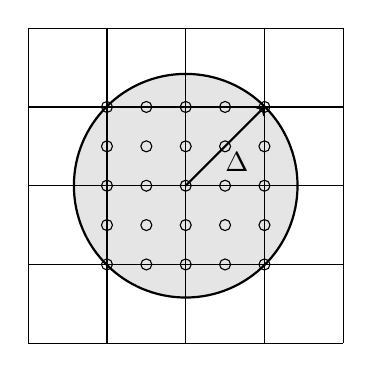
\begin{tikzpicture}
% cercle
\draw[thick,fill=black!10!] (2,2) circle (1.42);
% fleche
\tikz[overlay]\draw[thick,->] (2,2) -- (3,3); // flèche
\draw (2.65,2.3) node {$\Delta$};
% grille
\draw[step=1.0,black,thin] (0,0) grid (4,4);
% noeuds
\foreach \x in {1,1.5,...,3}
    \foreach \y in {1,1.5,...,3}
    {
    \draw (\x,\y) circle (0.07cm);
    }
\end{tikzpicture}
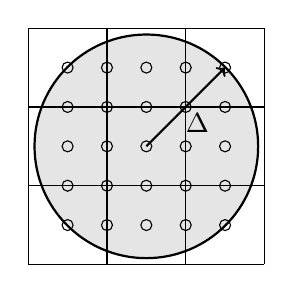
\begin{tikzpicture}
% cercle
\draw[thick,fill=black!10!] (1.5,1.5) circle (1.42);
% fleche
\tikz[overlay]\draw[thick,->] (1.5,1.5) -- (2.5,2.5); // fleche
\draw (2.15,1.8) node {$\Delta$};
% grille
\draw[step=1.0,black,thin] (0,0) grid (3,3);
% noeuds
\foreach \x in {0.5,1,...,2.5}
    \foreach \y in {0.5,1,...,2.5}
    {
    \draw (\x,\y) circle (0.07cm);
    }
\end{tikzpicture}
\caption{Filter zone (grey) in a regular mesh}
\label{fig:filterwidth}
\end{figure}

\begin{figure}[!ht]
\centering
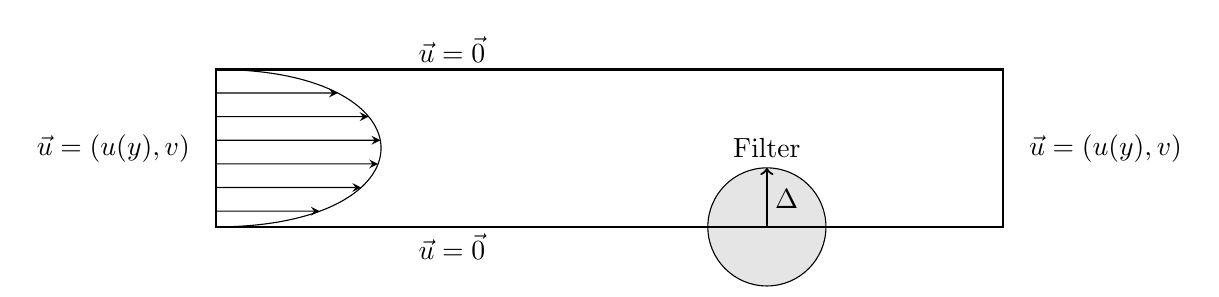
\begin{tikzpicture}
%  velocity profile
% found this method on stackoverflow somewhere :\ sorry for not citing.
\draw[name path=curve] (0,0)..controls(2.8,0) and (2.8,2) ..(0,2);% draw profile
\foreach \y in {0.2,0.5,...,2.0}{
    % horizontale invisible line
    \path[name path=horizontal] (0.2,\y) -- + (2.8,0);
    % than plot from (0, \y) to the intersection of the horizontale path
    % and the velocity profile
    \draw[-stealth,name intersections={of=curve and horizontal}] (0,\y) -- (intersection-1);
}
\draw (7,1) node {Filter};
\draw[fill=black!10!] (7,0) circle (.75); // cercle du filtre
\tikz[overlay]\draw[thick,->] (7,0) -- (7,.75); // flèche
\draw (7.25,0.35) node {$\Delta$};
\draw (-1.3,1) node {$\vec{u}=(u(y),v)$};
\draw (3,2.25) node {$\vec{u}=\vec{0}$};
\draw (11.3,1) node {$\vec{u}=(u(y),v)$};
\draw (3,-0.25) node {$\vec{u}=\vec{0}$};
\draw[thick] (0,0) rectangle (10,2);
\end{tikzpicture}
\caption{Velocity profile filter and boundary conditions}
\label{fig:filtrebord}
\end{figure}


% dimension style
\tikzset{%
    body/.style={inner sep=0pt,outer sep=0pt,draw,thick},
    dimen/.style={<->,>=latex,thin,every rectangle node/.style={fill=white,midway,font=\sffamily}},
    symmetry/.style={dashed,thin},
}

\begin{figure}[!ht]
\centering
\begin{tikzpicture}[scale=1.3]
% Specify the coordinates
\coordinate (A) at (0,0);
\coordinate (B) at (0,2);
\coordinate (C) at (1,2);
\coordinate (D) at (1,3);
\coordinate (E) at (9,3);
\coordinate (F) at (9,0);

\draw [body] (A) -- (B) -- (C) -- (D) -- (E) -- (F) -- (A);
\node[above] at ($ (B) !0.5! (C) $) {Inlet};
\node[rotate=90, above] at ($ (E) !0.5! (F)$) {Outlet};

% dimensions
\draw (A) -- ++(-0.5,0.0) coordinate (A1) -- +(0, 5pt);
\draw (B) -- ++(-0.5,0.0) coordinate (B1) -- +(0, -5pt);
\draw [dimen] (A1) -- (B1) node {$2D$};

\draw (A) -- ++(0,-0.5) coordinate (A2) -- +(5pt,0);
\draw (F) -- ++(0,-0.5) coordinate (F1) -- +(-5pt,0);
\draw [dimen] (A2) -- (F1) node {$20D$};

\draw (E) -- ++(0.5,0.0) coordinate (E1) -- +(0, -5pt);
\draw (F) -- ++(0.5,0.0) coordinate (F2) -- +(0, 5pt);
\draw [dimen] (E1) -- (F2) node {$3D$};

\draw (B) -- ++(0, 0.5) coordinate (B2) -- +(5pt, 0);
\draw (C) -- ++(0, 0.5) coordinate (C1) -- +(-5pt,0);
\draw [dimen,-] (B2) -- (C1) node [above=1pt] {$0.5D$};
\draw [dimen,<-] (B2) -- ++(-5pt,0);
\draw [dimen,<-] (C1) -- ++(+5pt,0);

% axe z
\coordinate (F3) at (10.1,1.1);
\draw[->] (F) -- (10.3, 1.3) node [above=1pt] {$z$};
\draw (F) -- ++(0.3,0.0) coordinate (F4);
\draw (F3) -- ++(0.3,0.0) coordinate (F31);
\draw [dimen] (F4) -- (F31) node {$w$};

% profil d'entree
\draw[name path=parabola] (0,1) parabola (C);
\foreach \x in {0.1, 0.3, ..., 0.9}{
   \path[name path=vertical] (\x, 2) -- + (0,-1);
   \draw[-stealth,name intersections={of=parabola and vertical}] (\x,2)  -- (intersection-1);
}

% symétrie
\draw[symmetry] (0,-1) --  (0, 4) node[anchor=north west] {axis};
\end{tikzpicture}
\caption{Géométrie du jet impactant}
\label{fig:jet2d}
\end{figure}

\begin{figure}[!ht]
\centering
\begin{tikzpicture}[scale=0.6]
% axis
\draw[thick,dashed,->] (-0.5, 0) -- (27, 0);
\draw[thick,->] (0,0.5) -- (0,-10);
\node at (26.5, 0.5) {$z$};
\node at (-0.5, -9.5) {$r$};

% arbre
\draw (0,0) rectangle (24, -2);
\node at (12.5, -1) {Arbre-hélice};

% bague d'acier
\draw  (6, -2) rectangle (10, -6);
\node[align=center] at (8, -4) {Bague\\Acier};

% bague graphite
\draw (10,-3) -- (15, -3) -- (15, -5.5) -- (12, -5.5) -- (12, -6) -- (10, -6) -- (10,-3);
\node[align=center] at (12.5, -4) {Bague\\Graphite};

% eau
\draw (10, -2) -- (10, -3) -- (15,-3) -- (15, -5.5) -- (24, -5.5) -- (24, -2) -- (10, -2);
\node at (19.5, -4) {Eau};

% joint nitrite
\draw  (12, -6) rectangle (24, -5.5);
\node at (18, -5.75) {Joint nitrite};

% Dimensions
% horizontales
\draw (0, -8) -- ++(0,-1) coordinate (A1) -- +(0, -5pt);
\draw (6, -8) -- ++(0,-1) coordinate (A2) -- +(0, -5pt);
\draw [dimen] (A1) -- (A2) node {$6$};

\draw (6, -8) -- ++(0,-1) coordinate (B1) -- +(0, -5pt);
\draw (10, -8) -- ++(0,-1) coordinate (B2) -- +(0, -5pt);
\draw [dimen] (B1) -- (B2) node {$4$};

\draw (10, -8) -- ++(0,-1) coordinate (C1) -- +(0, -5pt);
\draw (12, -8) -- ++(0,-1) coordinate (C2) -- +(0, -5pt);
\draw [dimen] (C1) -- (C2) node {$2$};

\draw (12, -8) -- ++(0,-1) coordinate (D1) -- +(0, -5pt);
\draw (24, -8) -- ++(0,-1) coordinate (D2) -- +(0, -5pt);
\draw [dimen] (D1) -- (D2) node {$12$};

\draw (10, -6.5) -- ++(0.0,-1) coordinate (E1) -- +(0, -5pt);
\draw (15, -6.5) -- ++(0.0,-1) coordinate (E2) -- +(0, -5pt);
\draw [dimen] (E1) -- (E2) node {$5$};

% verticales
\draw (25, 0) -- ++  (1,0) coordinate (F1) -- +(5pt, 0);
\draw (25, -2) -- ++(1,0) coordinate (F2) -- +(5pt, 0);
\draw [dimen] (F1) -- (F2) node {$2$};

\draw (25, -2) -- ++  (1,0) coordinate (G1) -- +(5pt, 0);
\draw (25, -5.5) -- ++(1,0) coordinate (G2) -- +(5pt, 0);
\draw [dimen] (G1) -- (G2) node {$3.5$};

\draw (25, -5.5) -- ++  (1,0) coordinate (H1) -- +(5pt, 0);
\draw (25, -6) -- ++(1,0) coordinate (H2) -- +(5pt, 0);
\draw [dimen] (H1) -- (H2);
\node at (26.75, -5.75) {$0.5$};

\draw (5.5, -3) -- ++(-1,0) coordinate (I1) -- +(-5pt, 0);
\draw (5.5, -6) -- ++(-1,0) coordinate (I2) -- +(-5pt, 0);
\draw [dimen] (I1) -- (I2) node {$3$};

% frontières
\node at (-0.5, -1) {$\Gamma_1$};
\node at (3, -2.5) {$\Gamma_2$};
\node at (5.5, -4) {$\Gamma_3$};
\node at (8, -6.5) {$\Gamma_4$};
\node at (11, -6.5) {$\Gamma_5$};
\node at (18, -6.5) {$\Gamma_6$};
\node at (24.5, -5.75) {$\Gamma_7$};
\node at (24.5, -3.75) {$\Gamma_8$};
\node at (24.5, -1) {$\Gamma_9$};
\node at (10.55, -4.5) {$\Gamma_{10}$};
\draw[color=red, ultra thick] (10, -6) -- (10,-3);
\end{tikzpicture}

\caption{Schéma du joint tournant}
\label{fig:geometrie}
\end{figure}

\begin{figure}[!ht]
\centering
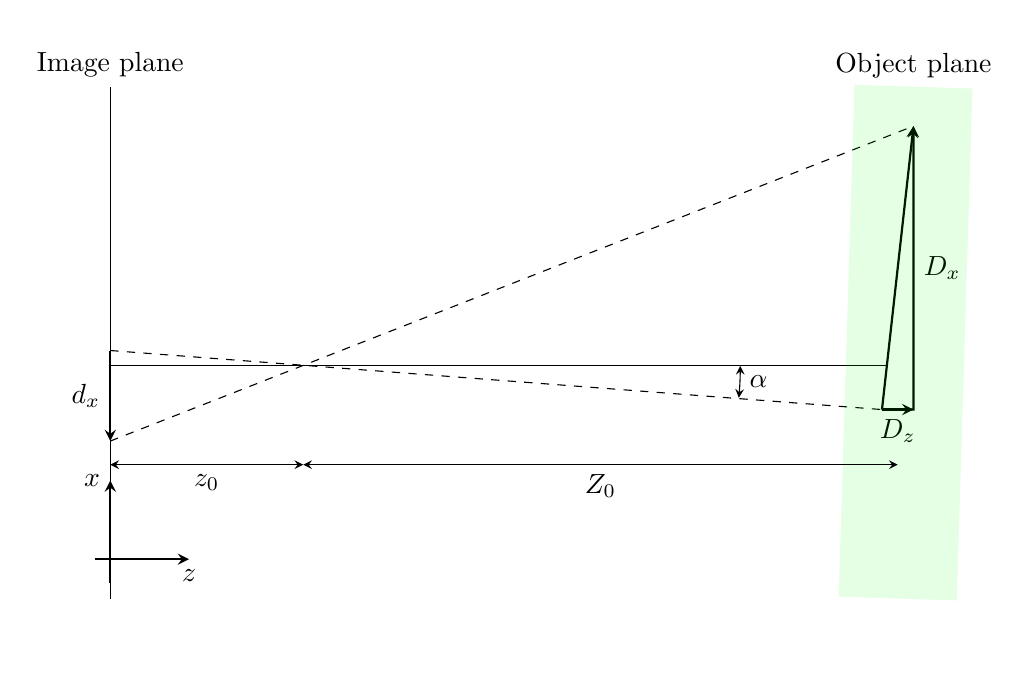
\begin{tikzpicture}[scale=1.0]

\pgfmathsetmacro{\xi}{0.15};
\pgfmathsetmacro{\Xi}{-0.6};
\pgfmathsetmacro{\xf}{-1};
\pgfmathsetmacro{\Xf}{3};
\pgfmathsetmacro{\Dz}{0.4};


% vectors
\draw[thick, ->, >=stealth] (0, \xi) -- (0, \xf) node[midway,left] {$d_x$};
\draw[thick, ->, >=stealth] (10-\Dz/2, \Xi) -- (10+\Dz/2, \Xf);
\draw[thick, ->, >=stealth] (10-\Dz/2, \Xi) -- +(\Dz, 0) node[midway,below] {$D_z$};
\draw[thick, ->, >=stealth] (10-\Dz/2, \Xi) -- +(\Dz, 0) -- (10+\Dz/2, \Xf) node[midway,right] {$D_x$};

% light paths
\draw[dashed] (0, \xi) -- (10-\Dz/2, \Xi);
\draw[dashed] (0, \xf) -- (10+\Dz/2, \Xf);

% planes
\draw (0,-0.045) -- (9.85,-0.045);
\draw[color=green, line width=1.5cm, opacity=0.1] (10,-3) -- (10+\Dz/2,3.5) node[black,opacity=1,above=-0.75cm] {Object plane};
\draw (0,-3) -- (0,3.5) node[above] {Image plane};

% axis
\draw[thick, ->, >=stealth] (0,-2.8) -- (0, -1.5) node[left] {$x$};
\draw[thick, ->, >=stealth] (-0.2,-2.5) -- (1, -2.5) node[below] {$z$};

% ratio lens
\draw[<->, >=stealth] (0, -1.3) -- (2.45, -1.3) node[midway, below] {$z_0$};
\draw[<->, >=stealth] (2.45, -1.3) -- (10, -1.3) node[midway, below] {$Z_0$};
\draw[<->, >=stealth] (8, -0.045) arc (0:-5:4.65) node[right, midway] {$\alpha$};
\end{tikzpicture}

\caption{Two dimensional PIV measurements}
\label{fig:2dpiv}
\end{figure}

\begin{figure}[!ht]
\centering
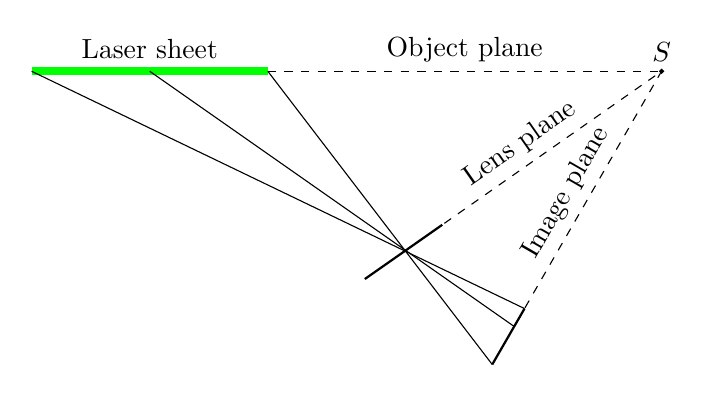
\begin{tikzpicture}[scale=1.0]

\pgfmathsetmacro{\plane}{3};
\pgfmathsetmacro{\lens}{1.2};
\pgfmathsetmacro{\sens}{0.82};
\pgfmathsetmacro{\dlens}{4};
\pgfmathsetmacro{\dsens}{3.89};
\pgfmathsetmacro{\dscheimpflug}{8};
\pgfmathsetmacro{\alens}{35};
\pgfmathsetmacro{\asens}{60};
\coordinate (Plane) at (\plane/2, 0);

\pgfmathsetmacro{\Lx}{\dscheimpflug-\dlens*cos(\alens)};
\pgfmathsetmacro{\Ly}{-\dlens*sin(\alens)};
\coordinate (Lens) at  (\Lx, \Ly);

\pgfmathsetmacro{\Sx}{\dscheimpflug-\dsens*cos(\asens)};
\pgfmathsetmacro{\Sy}{-\dsens*sin(\asens)};
\coordinate (Sensor) at (\Sx, \Sy);


\draw[color=green, line width=0.1cm] (0,0) -- node[color=black,above]{Laser sheet} (\plane,0);

% to intersection
\draw[fill, black] (\dscheimpflug, 0)  node[above]{$S$} circle [radius=0.025cm];
\draw[dashed] (\plane,0) --  node[above]{Object plane}  (\dscheimpflug, 0);
\draw[dashed] (Lens) -- node[above,rotate=\alens]{Lens plane} (\dscheimpflug, 0);
\draw[dashed] (Sensor) -- node[above,rotate=\asens] {Image plane} (\dscheimpflug, 0);

% draw lens and sensor
\draw[thick] (Lens) -- ++(\alens:\lens/2);
\draw[thick] (Lens) -- ++(180+\alens:\lens/2);
\draw[thick] (Sensor) -- ++(\asens:\sens/2);
\draw[thick] (Sensor) -- ++(180+\asens:\sens/2);
\draw (Sensor)+(\asens:\sens/2) -- (0,0);
\draw (Sensor)+(180+\asens:\sens/2) -- (\plane,0);
\draw (Plane) -- ++(-\alens:5.65);

\end{tikzpicture}

\caption{Scheimpflug condition}
\label{fig:scheimpflug_condition}
\end{figure}

\begin{figure}[!ht]
\centering
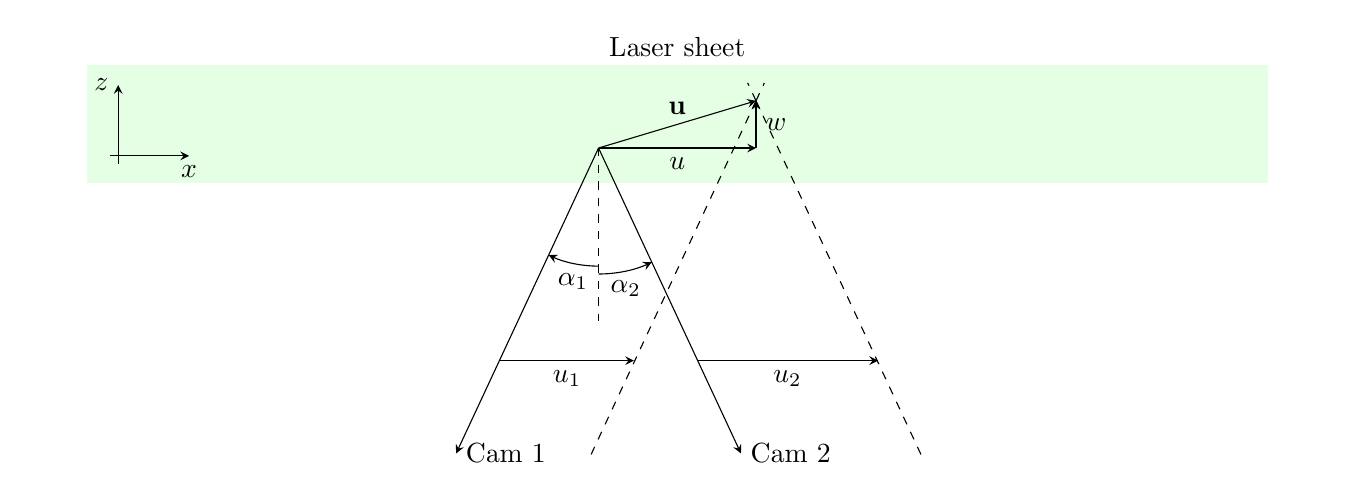
\begin{tikzpicture}[scale=1.0]
\pgfmathsetmacro{\plane}{15};
\draw[color=green, line width=1.5cm, opacity=0.1] (0,0) -- node[color=black,above,opacity=1.0]{Laser sheet} (\plane,0);

\pgfmathsetmacro{\dx}{2.0};
\pgfmathsetmacro{\dy}{0.6};
\coordinate (particle) at (6.5, -0.3);

\draw[->,>=stealth] (particle) -- node[above]{$\v u$} +(\dx, \dy);
\draw[->,>=stealth] (particle) -- node[below]{$u$} +(\dx, 0);
\draw[->,>=stealth] (particle)+(\dx,0) -- node[right]{$w$} ($(particle) + (\dx,\dy)$);

% axis
\draw[->,>=stealth] (0.3, -0.4) -- +(1, 0) node[below] {$x$};
\draw[->,>=stealth] (0.4, -0.5) -- +(0, 1) node[left] {$z$};

% projection
\draw[->,>=stealth] (particle) -- +(180+65:4.28) node[right] {Cam 1};
\draw[dashed] ($(particle)+(\dx,\dy)$) -- ++(65:0.25);
\draw[dashed] ($(particle)+(\dx,\dy)$) -- ++(180+65:5);

\draw[->,>=stealth] (particle) -- +(180+115:4.28) node[right] {Cam 2};
\draw[dashed] ($(particle)+(\dx,\dy)$) -- ++(115:0.25);
\draw[dashed] ($(particle)+(\dx,\dy)$) -- ++(180+115:5);

% angle
\draw[dashed] (particle) -- +(0, -2.2);
\draw[->,>=stealth] (particle)+(0, -1.5) arc (270:180+65:1.5) node[below, midway] {$\alpha_1$};
\draw[->,>=stealth] (particle)+(0, -1.6) arc (270:180+115:1.6)node[below, midway] {$\alpha_2$};

% velocity cam
\draw[->,>=stealth] (5.25, -3) -- node[below] {$u_1$} +(1.7, 0);
\draw[->,>=stealth] (7.75, -3) -- node[below] {$u_2$} +(2.3, 0);
\end{tikzpicture}

\caption{Stereo method}
\label{fig:polaro}
\end{figure}

%=== PROFIL DE VITESSE ET COUCHE DE DIFFUSION===%
\begin{figure}[!ht]
\centering
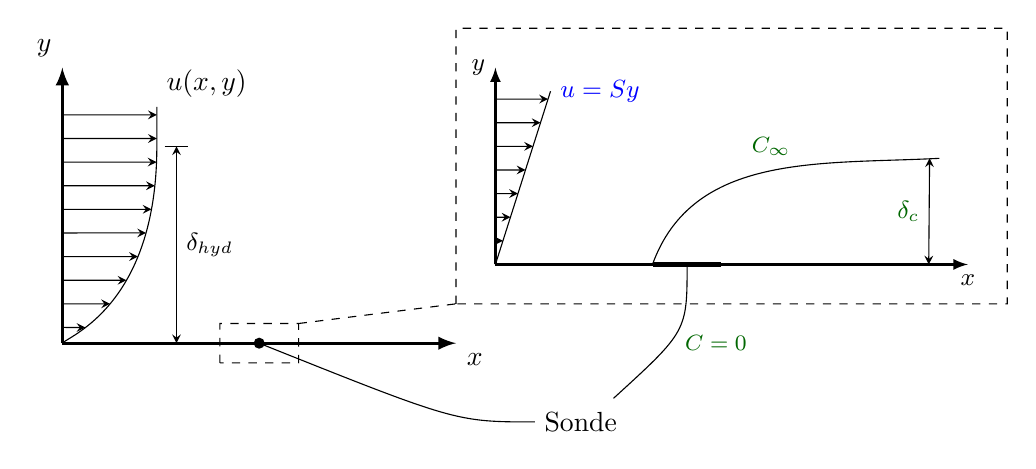
\begin{tikzpicture}
\def\ymax{3}
\def\xmax{5}

% Les axes et la sonde
\draw[very thick,->,>=latex] (0,0) -- (\xmax,0) node[below right] {$x$};  
\draw[very thick,->,>=latex] (0,0) -- (0,\ymax+.5) node[above left] {$y$};
\fill (\xmax/2,0) circle (2pt);

% Profil de vitesse
\draw[name path=curve] (0,0)..controls(0.1,0.1) and (1.2,0.5)  ..(1.2,\ymax-.5) -- (1.2,\ymax) node[above right] {$u(x,y)$};
\foreach \y in {0.2,0.5,...,\ymax}{
	\path[name path=horizontal] (0,\y) -- + (2,0);
	\draw[-stealth,name intersections={of=curve and horizontal}] (0,\y) -- (intersection-1);
}

% delta hydro
\draw (1.3,\ymax -.5) -- (1.6,\ymax-.5);
\draw[<->,>=stealth] (1.45,0) -- node[right] {\small $\delta_{hyd}$} (1.45,\ymax-.5);

% Zoom
\draw[dashed] (\xmax/2-.5,-.25) rectangle (\xmax/2+.5,0.25) -- (\xmax,0.5) rectangle + (7,3.5) ;

% Nouvels axes et sonde
\draw[->,thick,>=latex]  (\xmax+.5,\ymax/3)  -- node (A) {} +  (6,0) node[pos=0.917,below] (D) {} node[below] {\small $x$};
\draw[->,thick,>=latex] (\xmax+.5,\ymax/3) -- (\xmax+.5,\ymax+.5) node[left] {\small$y$};
\draw[line width=2pt] (A) -- node[above] (AA) {} +(-1,0) node[pos=1.07,below] (B) {};

% Couche de diffusion
\draw (B) to [out=70, in=183] + (3.7,1.5) node[above left] (C) {};
\draw[<->,>=stealth] (C) -- node[left] {\small $\color{green!40!black}\delta_c$} (D);
\draw (8.3,0) node{\footnotesize$\color{green!40!black}C=0$};
\draw (9,2.5) node{\footnotesize$\color{green!40!black}C_\infty$};

% Profil linéaire    
\draw[name path=curve1] (\xmax+.5,\ymax/3) -- (\xmax+1.2,\ymax+.2) node[right]{\small$\color{blue}u=Sy$};    
\foreach \y in {1.3,1.6,...,3.2}{
	\path[name path=horiz] (\xmax+.5,\y) -- + (3,0);
	\draw[-stealth,name intersections={of=curve1 and horiz}] (\xmax+.5,\y) -- (intersection-1);
}

% Notes
\draw (AA)[left]..controls +(0,-1).. (\xmax+2,-0.7);
\draw(\xmax+1,-1) node[right] {Sonde}..  controls (\xmax,-1) ..(\xmax/2,0);
\end{tikzpicture}
\end{figure}

%=== SONDES POLARO ===%
\begin{figure}[!ht]
\centering
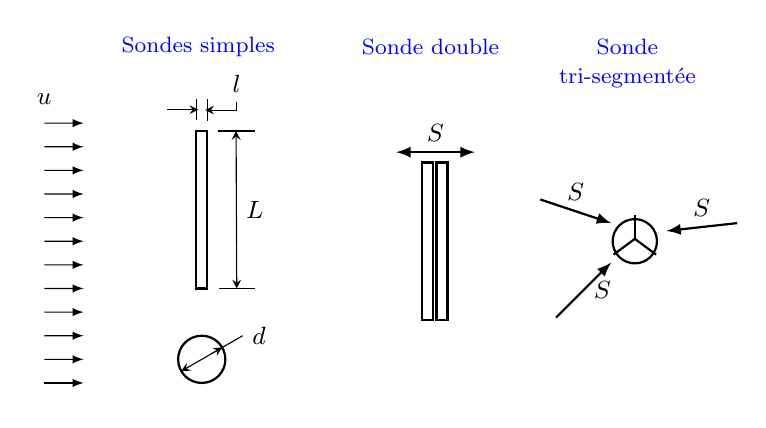
\begin{tikzpicture}
\tikzstyle{every node}=[font=\footnotesize]
\def\ymax{3.6}
\def\xmax{4}
\def\ray{0.3}

% Vitesse
\path[name path=curve1] (0.5,0) -- (0.5,\ymax);
\draw (0,\ymax) node {\small$u$} ;
\foreach \y in {0,0.3,...,\ymax}{
	\path[name path=horiz1] (0,\y) -- + (3,0);
	\draw[-latex,name intersections={of=curve1 and horiz1}] (0,\y) -- (intersection-1);
}
% Pour voir la flèche du bas
\draw (0,-0.1) node{};


%=== Sondes simples
\draw[thick] (2,0.3) node (B){} circle (\ray) ;    
\draw[thick] (1.93,1.2) rectangle (2.07,3.2) node (A) {};

% Distance L
\draw (A) -- node[above] (AA){} + (0.6,0);
\draw ($(A)-(-0.15,2)$) -- node[below] (BB){} + (0.45,0);
\draw[<->,>=stealth] (AA) -- node[right] {\small $L$} (BB);
% Distance l
\draw (A) -- node[right] (CC){} +(0,0.4);
\draw ($(A)-(0.14,-0.14)$) -- node[left] (DD){} +(0,0.26);
\draw[<-,>=stealth] ($(CC)-(0.15,0)$) -|+ (0.4,0.1) node[above] {\small$l$};
\draw[<-,>=stealth] ($(DD)+(0.15,0)$) -- + (-0.4,0);
% Diamètre d
\draw[<->,>=stealth] ($ (B) - (0.866*\ray,\ray*0.5) $) -- node (C){} ($(B) + (0.866*\ray,\ray*0.5)$)  ;
\draw (C) --+ ($2*(0.866*\ray,\ray*0.5)$) node[right] {\small $d$}; 
% Titre
\node at ($(DD)+(0.15,0.8)$) {\color{blue} Sondes simples};


%=== Sonde double
\draw[thick] (4.8,0.8) rectangle+ (0.14,2) node[above left](top) {};
\draw[thick] (4.98,0.8) rectangle+ (0.14,2) node {};
% S
\draw[thick,<->,>=latex] ($(top)-(0.34,0)$) -- node[above]{\small$S$} +(1,0);
% Titre
\node at ($(DD)+(3.1,0.8)$) {\color{blue} Sonde double};


%=== Sonde triseg
\draw[thick] (7.5,1.8) circle  (0.8em);
    \newcommand{\y}{1.83}
    \newcommand{\x}{7.5}
\draw[thick] (\x,\y) -- +(0,.3);
\draw[thick] (\x,\y) -- +(0.27,-.2);
\draw[thick] (\x,\y) -- +(-0.27,-.2);
% S
\draw[->,>=latex,thick] (\x-1,\y-1) -- node[right] {\small $S$} + (0.7,0.7) ;
\draw[->,>=latex,thick] (\x-1.2,\y+0.5) -- node[above] {\small $S$} + (0.9,-0.3) ;
\draw[->,>=latex,thick] (\x+1.3,\y+0.2) -- node[above] {\small $S$} + (-0.9,-0.1) ;
% Titre
\node at ($(DD)+(5.6,0.8)$) {\color{blue} Sonde};
\node at ($(DD)+(5.6,0.4)$) {\color{blue} tri-segmentée};
\end{tikzpicture}
\end{figure}

\end{document}